\input /Users/davidmcallester/ICloude/tex/SlidePreamble
\input /Users/davidmcallester/ICloude/tex/preamble


\begin{document}

{\Huge

  \centerline{\bf TTIC 31230, Fundamentals of Deep Learning}
  \bigskip
  \centerline{David McAllester, Autumn 2021}
  \vfill
  \vfil
  \centerline{Vector Quantized Variational Autoencoders (VQ-VAEs)}
  \vfill
  \vfill

\slide{Gaussian VAEs for Faces 2014}

We can sample faces from the VAE by sampling noise $z$ from $p_\Phi(z)$ and then sampling an image $y$ from $p_\Phi(y|z)$.

\vfill
\centerline{\includegraphics[width = 3in]{\images/VariationalFaces}}
\centerline{[Alec Radford]}

\slide{VQ-VAEs 2019}

\centerline{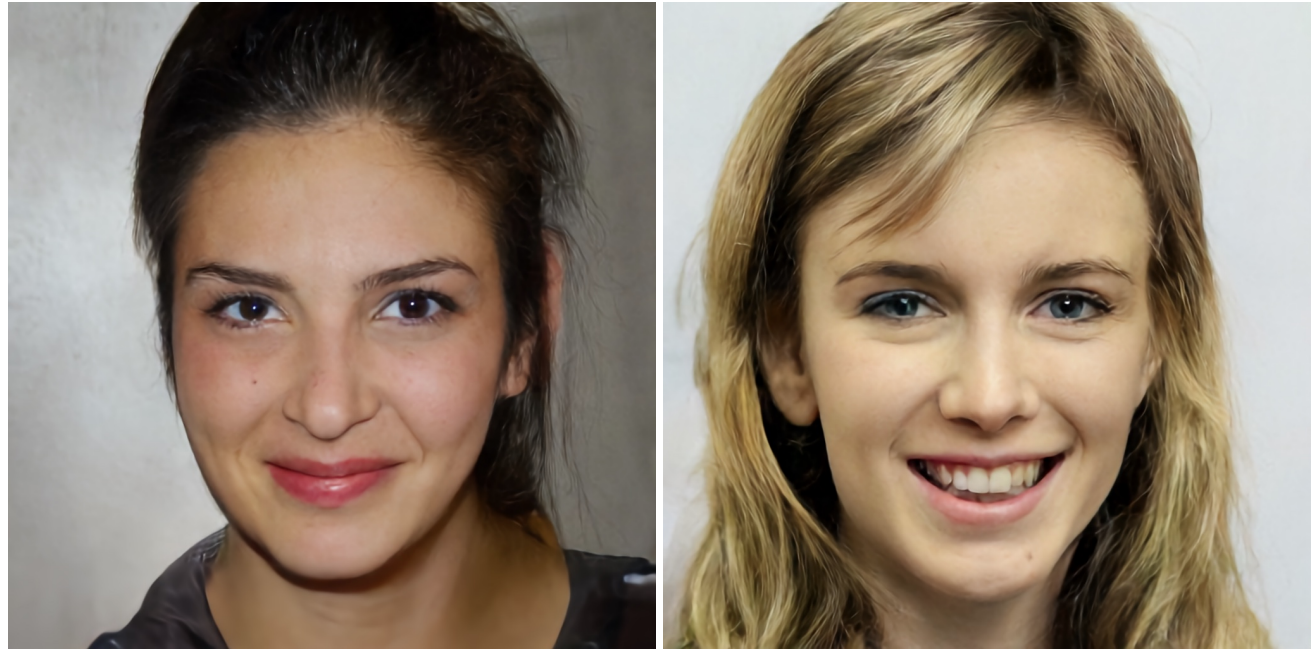
\includegraphics[width = 8in]{\images/VQ-VAE22}}

\vfill
VQ-VAE-2, Razavi et al. June, 2019

\slide{VQ-VAEs 2019}

\centerline{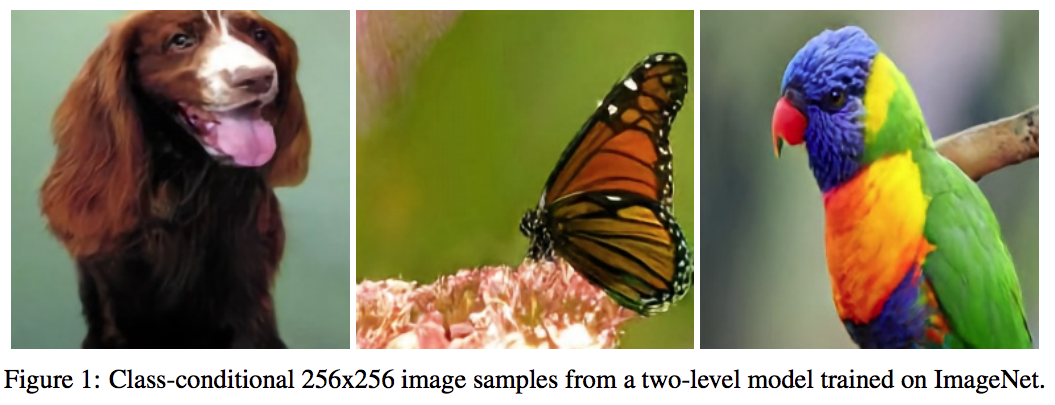
\includegraphics[width = 10in]{\images/VQ-VAE21}}

\vfill
VQ-VAE-2, Razavi et al. June, 2019


\slide{The VQ Recipe}

{\huge
This is an abstraction of the methodology used in vector quantized VAEs.

$$\Psi^*,\Theta^* = \argmin_{\Psi,\Theta} E_{y \sim \pop,\;z \sim P_\Psi(z|y)}\left[{\cal L}_{\mathrm{enc}}(\Psi,z,y) \;-\;\ln P_\Theta(y|z)\right]$$

\vfill
Since the loss ${\cal L}_{\mathrm{enc}}(\Psi,z,y)$ depends only on the encoder we have

$$\Theta^* = \argmin_\Theta\;E_{y \sim \pop,z \sim P_{\Psi^*}(z|y)}\left[-\ln P_\Theta(y|z)\right]$$

Then train $\Phi$ by

\begin{eqnarray*}
\Phi^* &  = & \argmin_{\Phi}\;E_{y\sim \pop,z\sim P_{\Psi^*}(z|y)}\left[-\ln P_\Phi(z)\right]
\end{eqnarray*}
}


\slide{The VQ Recipe}

{\huge

$$\Theta^* = \argmin_\Theta\;E_{y \sim \pop,z \sim P_{\Psi^*}(z|y)}\left[-\ln P_\Theta(y|z)\right]$$

\begin{eqnarray*}
\Phi^* &  = & \argmin_{\Phi}\;E_{y\sim \pop,z\sim P_{\Psi^*}(z|y)}\left[-\ln P_\Phi(z)\right]
\end{eqnarray*}

\vfill
Under a universality assumption for $\Phi$ and $\Theta$ we have that a perfect model of $y$ can be achieved by optimizing the prior $P_\Phi(z)$ in a final pass for pre-trained $\Psi$ and $\Theta$.

\vfill
Joint Training of $\Phi$ with $\Psi$ and $\Theta$ is not required.

}

\slide{VQ-VAE-2 Image Model}


Here we present a rational reconstruction and simplification of the VQ-VAE-2.


\centerline{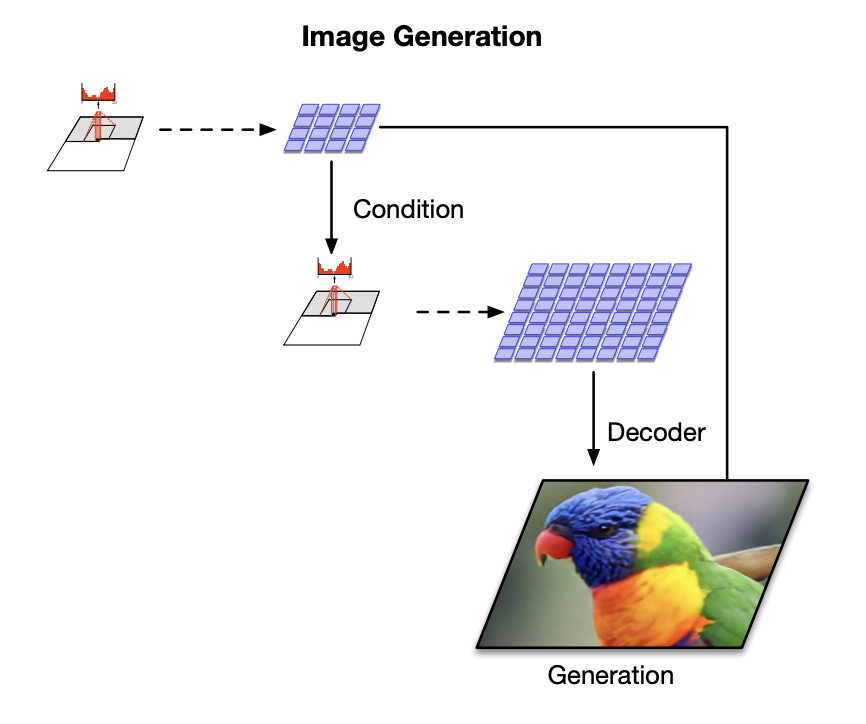
\includegraphics[height =2in]{\images/VQSampler} \parbox[b]{1.0in}{\Large $z_2$ \\ \\ $z_1$ \\ \\ $y$ \\ \\ ~}}

\vfill
In the multi-resolution case (similar to progressive GANs) we train a finest resolution VAE first with latent variable $z_1$.

\vfill
We then model $P(z_1)$ recursively using a coarser resolution latent variable $z_2$ and so on.

\slide{VQ-VAE Image Model}

\centerline{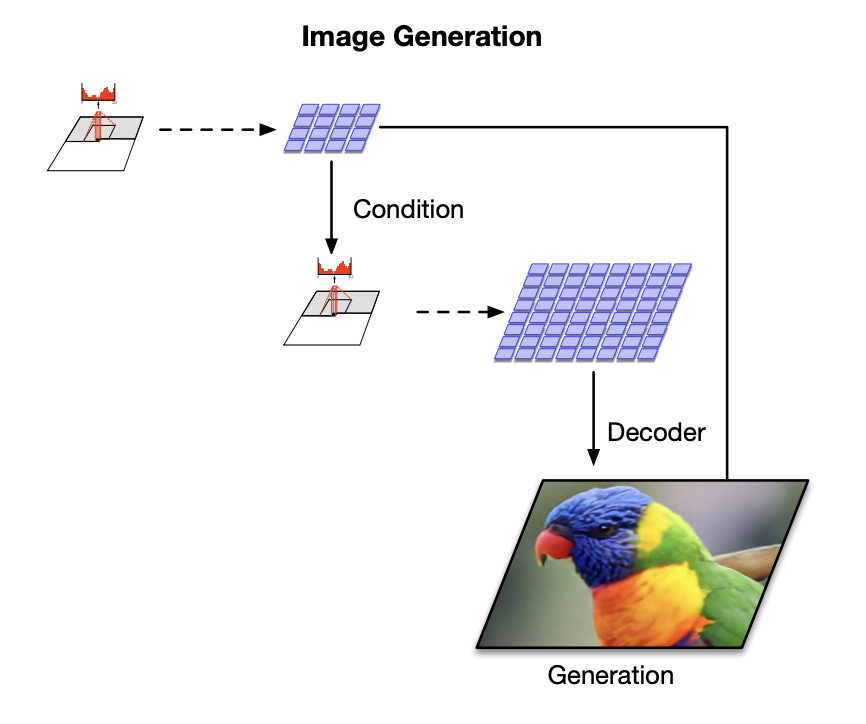
\includegraphics[height =2in]{\images/VQSampler} \parbox[b]{1.0in}{\Large $z_2$ \\ \\ $z_1$ \\ \\ $y$ \\ \\ ~}}

\vfill

At each layer $z_i$ is a ``symbolic image'' --- each pixel is assigned a symbol --- and the $P(z_i)$ is an auto-regressive model
analogous to a language model.

\slide{VQ-VAE Image Model}

\centerline{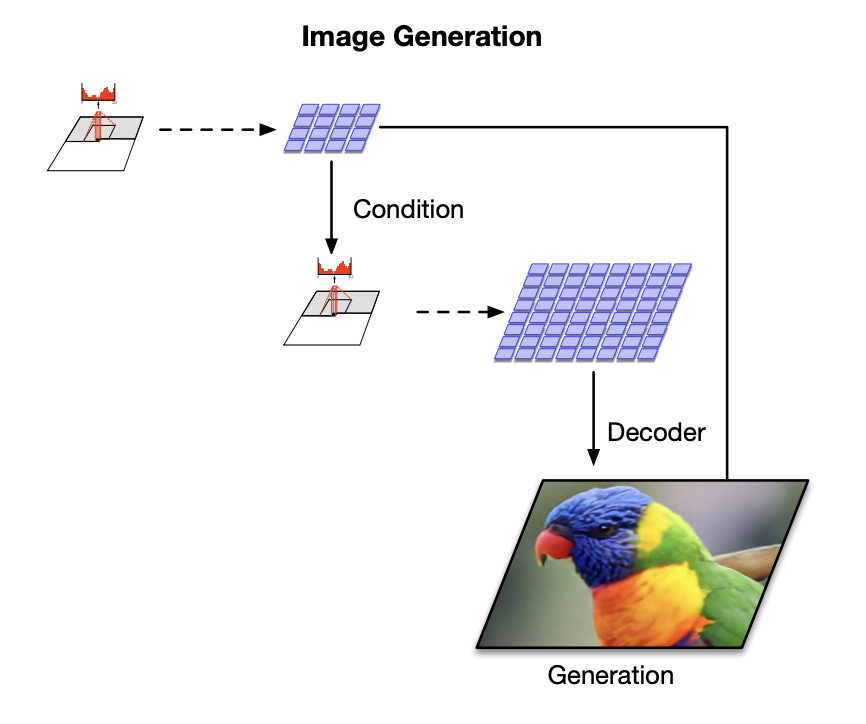
\includegraphics[height =2in]{\images/VQSampler} \parbox[b]{1.0in}{\Large $z_2$ \\ \\ $z_1$ \\ \\ $y$ \\ \\ ~}}

\vfill
Each layer can use the same training recipe except that in the first layer $y$ is continuous.

\vfill
This gives  $-\log_2 P_\Phi(z[X,Y])$ bits per image (much lower).

\vfill
To sample an image they sample $z[X,Y]$ from $P_\Phi(z[X,Y])$.


\slide{VQ-VAE Training}

We wish to model $s$ where $s$ is either the image or a coarser symbolic image of a previous layer.

\vfill
We have an encoder network, such as a CNN, which produces a layer with a vector at each pixel position.

\begin{eqnarray*}
L[X,Y,I] & = & \mathrm{Enc}_\Phi(s) \\
\end{eqnarray*}

Intuitively we cluster the vectors $L(x,y,I)$ using K-means clustering to produce cluster centers where $C[k,I]$
is the cluster center vector of cluster $k$.

\slide{VQ-VAE Training}

We then replace each vector $L[x,y,I]$ by the nearest cluster center to give $\hat{L}[X,Y,I]$.

{\huge
\begin{eqnarray*}
z[x,y] & = & \argmin_k \;||L[x,y,I] - C[k,I]|| \\
\\
\hat{L}[x,y,I] & = & C[z[x,y],I] \\
\end{eqnarray*}
}

The ``symbolic image'' $z[X,Y]$ is the latent variable.

\slide{VQ-VAE Training}

Finally we decode $\hat{L}[X,Y,I]$ with a model $P_\Theta(s|z)$.

\slide{Training the Code Book}

We then apply the first step of the training recipe to the following loss function.

{\huge
\begin{eqnarray*}
\Psi^*,\Theta^* & = & \argmin_{\Psi,\Theta} \;E_{s\sim \pop,z\sim P_\Psi(z|s)}\left[ \frac{\beta}{2}||L[X,Y,I] - \hat{L}[X,Y,I]||^2 -\ln P_\Theta(s|z)\right]
\end{eqnarray*}
}

\vfill
Here the first term of the loss depends only on the encoder (no dependence on the decoder).

\slide{Handling Discrete Latents}


{\huge
\begin{eqnarray*}
z[x,y] & = & \argmin_k \;||L[x,y,I] - C[k,I]|| \\
\\
\hat{L}[x,y,I] & = & C[z[x,y],I]
\end{eqnarray*}
}

Since $z[x,y]$ is discrete we have $z[x,y].\grad = 0$.
They use ``straight-through'' gradients and ``k-means'' gradients.

{\huge
\begin{eqnarray*}
L[x,y,I].\grad & = & \hat{L}[x,y,I].\grad + \beta(L[x,y,I] - C[z[x,y],I]) \\
\\
C[k,I].\grad & = & \sum_{z[x,y]=k} \gamma(C[k,I] - L[x,y,I])
\end{eqnarray*}
}

\slide{Quantitative Evaluation}

The VQ-VAE2 paper reports a classification accuracy score (CAS) for class-conditional image generation.

\vfill
We generate image-class pairs from the generative model trained on the ImageNet training data.

\vfill
We then train an image classifier from the generated pairs and measure its accuracy on the ImageNet test set.

\vfill
\centerline{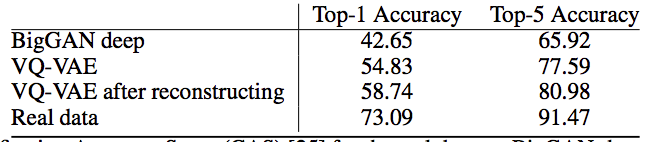
\includegraphics[width=7in]{\images/VQ-VAE23}}

\slide{Image Compression}

\vfill
\centerline{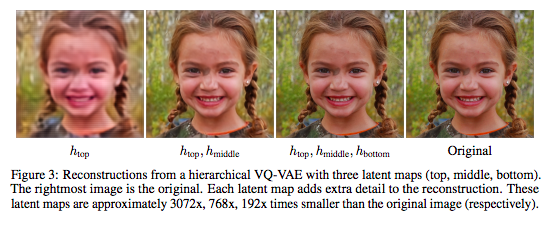
\includegraphics[width = 10in]{\images/VQgirl}}

\slide{Rate-Distortion Evaluation.}

Rate-distortion metrics for image compression to discrete representations support unambiguous rate-distortion evaluation.

\vfill
Rate-distortion metrics also allow one to explore the rate-distortion trade-off.

\vfill
\centerline{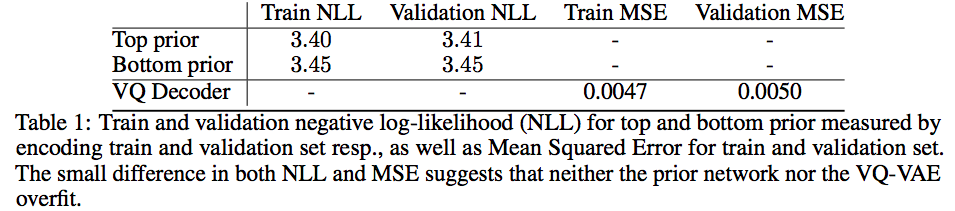
\includegraphics[width = 10in]{\images/VQVAE2Scores}}

\slide{DALL$\cdot$E: A Text-Conditional Image dVAE}
\vfill
DALL$\cdot$E is a text-conditional VQ-VAE model of images.

\vfill
The Vector quantization is done independent of the text.  However, the model of the probability distribution of the symbolic image $z[x,y]$ is conditioned on text.

\vfill
\centerline{\huge Ramesh et al. 2021}

\slide{DALL$\cdot$E}

\centerline{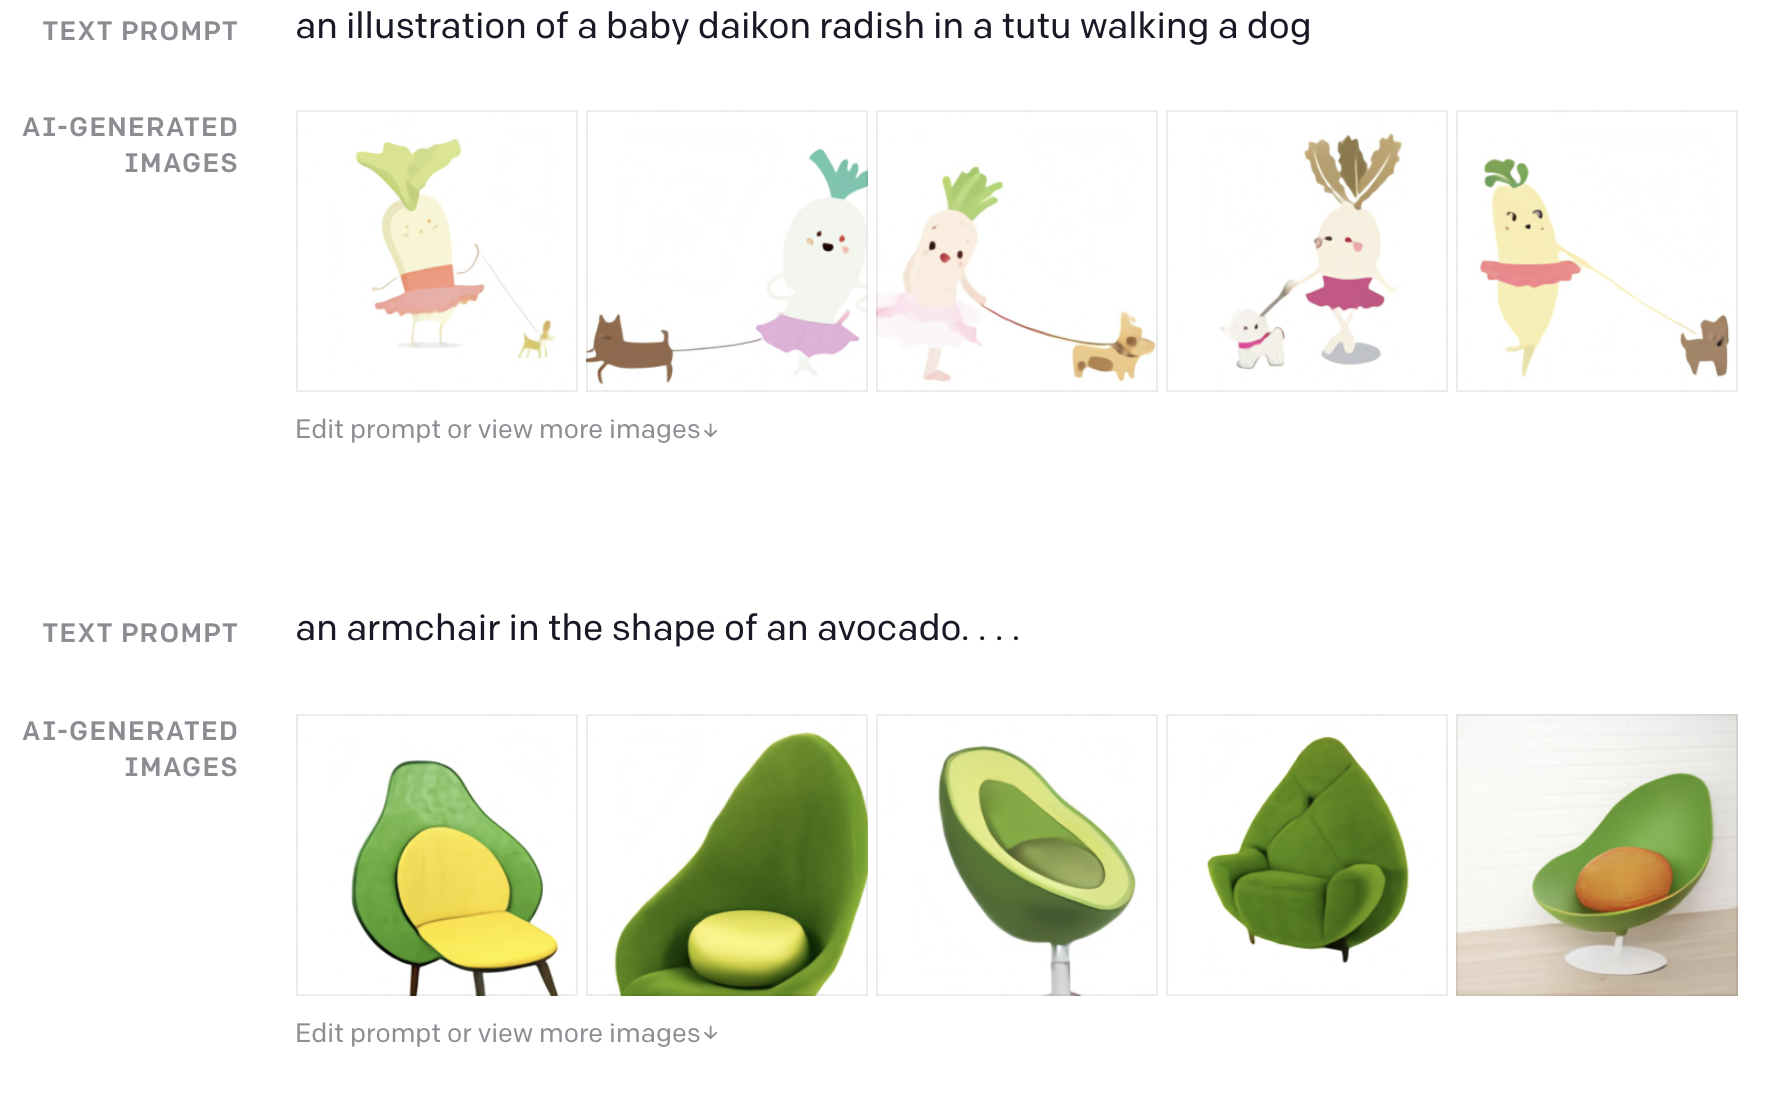
\includegraphics[height= 5.5in]{\images/DALLE1}}

\slide{Vector Quantized VAEs (VQ-VAE)}

VQ-VAEs effectively perform $k$-means on vectors in the model so as to represent vectors by discrete cluster centers.

\vfill
We use $x$ and $y$ for spatial image coordinates and use $s$ (for signal) to denote images.

\slide{VQ-VAE Encoder-Decoder}

\centerline{\includegraphics[width =5in]{\images/VQCodes}}

\vfill
In the one-layer case the latent variable (compressed image) is a ``symbolic image'' $z[X,Y]$ where $z[x,y]$ is a symbol (a cluster index).

\vfill
Naively $z[X,Y]$ can be represented with $XY \log_2 K$ bits.

\slideplain{END}

\end{document}
